\documentclass[10pt,a4paper]{report}
\usepackage[utf8]{inputenc}
\usepackage[russian]{babel}
\usepackage[OT1]{fontenc}
\usepackage{amsmath}
\usepackage{amsfonts}
\usepackage{amssymb}
\usepackage{graphicx}
\author{Киселев Антон и Кенть Никита}
\title{Отчет по лабораторной работе по дисциплине: "Сети и системы передачи данных"\newline
}
\date{13.03.14}
\begin{document}
\maketitle
\pagebreak
\chapter {Визуализация сигналов во временной и частотной области}
\section{Цель работы}
Познакомиться со средствами генерации сигналов и визуализации их спектров.
\section{Постановка задачи}
В командном окне MATLAB и в среде Simulink промоделировать чистый синусоидальный сигнал, 
так же синусоидальный сигнал с шумом. Получить их спектры.

\section{Теоретическая часть}
В ходе данной лабораторной работы необходимо промоделировать чистый синусоидальный сигнал, а так же синусоидальный сигнал с шумом и получить их представления во временной и частотной областях. Синусоидальный сигнал задаётся по следующей формуле: 
\begin{displaymath}
A(t) = A_0 * sin(2*\pi *f*t + u_0)
\end{displaymath}
Для создания зашумленного синусоидального сигнала, к чистому синусоидальному сигналу прибавляется случайная составляющая, по формуле:
\begin{displaymath}
A(t) = A_0 * sin(2*\pi *f*t + u_0) + A_1*rand()
\end{displaymath}
Для выделения частот регулярных составляющих сигнала необходимо использовать преобразование Фурье, реализуемое следующей формулой:
\begin{displaymath}
X(k) = \sum_{j=1}^N x(j)*e^{2*\frac{x}{N(j-1)(k-1)}}
\end{displaymath}
\section{Алгоритм работы. Построение сигналов}
\begin{itemize}
\item Построение синусоидального сигнала без шумов
\item Вывод временной характеристики сигнала
\item Реализация  преобразования Фурье 
\item Построение графика спектральной плотности 
\item Построение зашумленного синусоидального сигнала  
\item Вывод временной характеристики полученного сигнала
\item Преобразования Фурье 
\item Построение графика спектральной плотности для зашумленного сигнала
\end{itemize}
\section{Код MATLAB}
function main()\newline
x=0:0.01:4*pi;\newline
t0 = 5;\newline
\%исходный сигнал\newline
y = sin(2*pi*f0*x);\newline
figure(1)\newline
plot(x(1:200),y(1:200))\newline
grid\newline
\%спектр исходного сигнала\newline
figure(2)\newline
spectrum = fft(y,1024);\newline
normspectrum = spectrum.*conj(spectrum)/1024;\newline
f=100*(0:1023)/1024;\newline
plot(f, normspectrum(1:1024))\newline
axis([0 max(f) 0 10])\newline
grid\newline
\%зашумленный сигнал\newline
ynoize = y+ 0.5*rand(size(x));\newline
figure(3)\newline
plot(x(1:200),ynoize(1:200));\newline
grid\newline
\%спектр зашумленного сигнала\newline
spectrum = fft(ynoize,1024);\newline
noizespectrum = spectrum.*conj(spectrum)/1024;\newline
figure(4)\newline
plot(f, noizespectrum())\newline
axis([0 max(f) 0 10])\newline
grid\newline
\section{Результаты работы}
В результате выполнения программы получились графики временной и частотной характеристик исходного и зашумленного синусоидальных сигналов. \newpage
\begin{figure}
\begin{center}
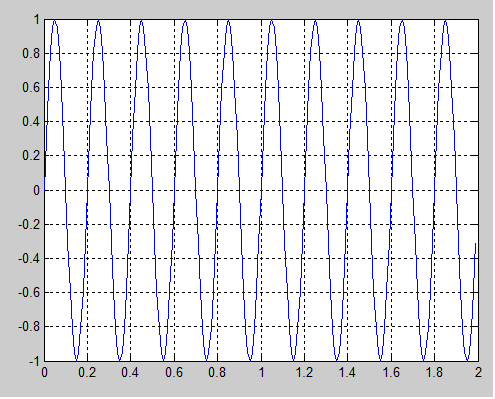
\includegraphics[angle=0, scale = 0.9]{1.png}\newline
рис. 1 Исходный сигнал\newline
\end{center}
\begin{center}
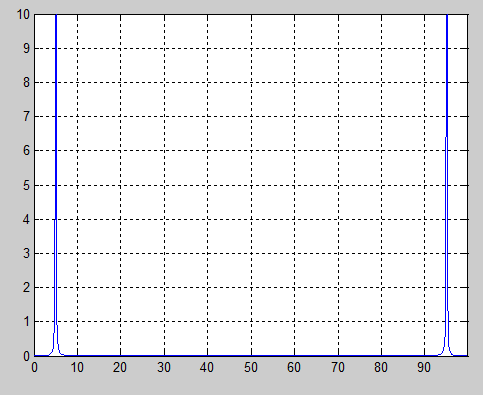
\includegraphics[angle=0, scale = 0.9]{2.png}\newline
рис. 2. Спектр исходного сигнала\newline
\end{center}
\end{figure}
\begin{figure}
\begin{center}
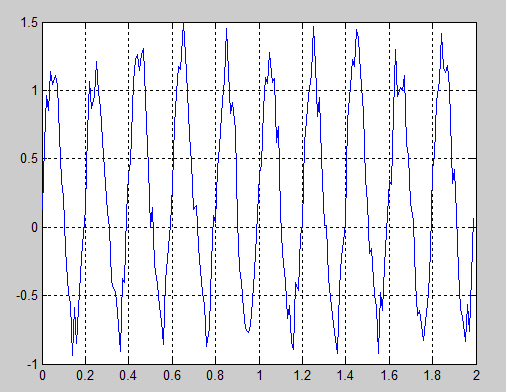
\includegraphics[angle=0, scale = 0.9]{3.png}\newline
рис. 3. Зашумленный сигнал\newline
\end{center}
\begin{center}
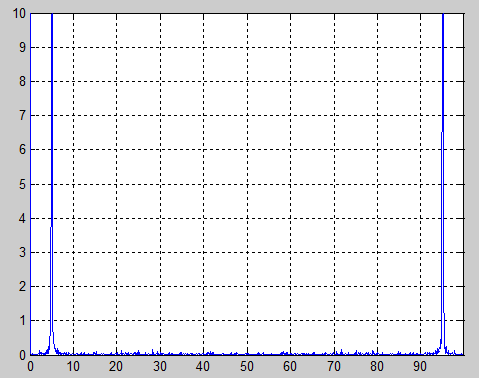
\includegraphics[angle=0, scale = 0.9]{4.png}\newline
рис. 4. Спектр зашумленного сигнала\newline
\end{center}
\end{figure}
\clearpage
\section{Вывод}
В данной лабораторной работе было проведено исследование по получению и сравнению спектров чистого и зашумленного сигнала. Спектры сигналов вычислялись на ограниченном промежутке. 
Для этого длина промежутка и частота квантования выбирались так, чтобы результаты вычислений были достаточно точными. Полученные результаты при вычислении спектра оказались ожидаемыми.
Теоретически ожидалось получить периодический спектр синусоидального сигнала как один импульс. Вследствие дискретности исходного сигнала, при выполнении операции по получению спектра,
синусоидальный сигнал умножается на на решетку дельта-импульсов. Происходит свертка исходного сигнала с решеткой дельта-импульсов. Поэтому при практическом опыте был получен
периодический спектр исходного сигнала, предщсталенный в виде нескольких импульсов на графике.. \newline

\chapter{Построение спектров}
\section{Алгоритм работы}
\begin{itemize}
\item Построение полигармонического сигнала
\item Построение прямоугольного импульсного сигнала
\item Построение треугольного импульсного сигнала
\item Получение спектров этих сигналов
\item Создание моделей в Simulink
\end{itemize}
\section  {Теоретическая часть}
В данной работе мы рассматриваем три типа сигналов: полигармонический, прямоугольный импульсный и треугольный. Их формулы представленны ниже:
\begin{itemize}
\item полигармонический сигнал 
\end{itemize}
\begin{displaymath}
y(t) = \sum_{n=0}^N-1 cos(nt)
\end{displaymath}
\begin{itemize}
\item прямоугольный импульсный сигнал
\end{itemize}
\begin{displaymath}
y(t) = \Pi (t,T_i)
\end{displaymath}
\begin{itemize}
\item треугольный импульсный сигнал
\end{itemize}
\begin{displaymath}
y(t) = \Delta (t,T_i)
\end{displaymath}
Для получения треугольного сигнала используется операция свертки двух прямоугольных сигналов, производимая по формуле:
\begin{displaymath}
(f*g)(x) = int_inf^-inf f(y)g(x-y)dy
\end{displaymath}
\section{Код MATLAB}
function laba5()\newline
x = 0:0.01:4*pi;\newline
f0 = 5;\newline
y = 0;\newline
for i=1:1:100\newline
    y=y+cos(i*x);\newline
end\newline
plot(x(1:100),y(1:100));\newline
figure(1)\newline
spectrum=fft(y,512);\newline
normspectrum=spectrum.*conj(spectrum)/512;\newline
f=100*(0:255)/512;\newline
figure(2)\newline
plot(f,normspectrum(1:256))\newline
axis([0 max(f) 0 10])\newline
grid \newline
figure(3)\newline
y1=square(x,50)\newline
plot(x(1:1000),y1(1:1000),'LineWidth',2);\newline
ylim([-1.2,1.2]);\newline
spectrum=fft(y1,512);\newline
normspectrum=spectrum.*conj(spectrum)/512;\newline
f1=100*(0:255)/512;\newline
figure(4)\newline
plot(f1,normspectrum(1:256))\newline
axis([0 max(f1) 0 10])\newline
grid \newline
y2=conv(y1,y1);\newline
figure(5)\newline
plot(x(1:1000),y2(1:1000),'LineWidth',2);\newline
grid\newline
spectrum=fft(y2,512);\newline
normspectrum=spectrum.*conj(spectrum)/512;\newline
f2=100*(0:255)/512;\newline
figure(6)\newline
plot(f2,normspectrum(1:256)/1000)\newline
axis([0 max(f2) 0 10])\newline
grid \newline
end\newline
\clearpage

\begin{figure}
\begin{center}
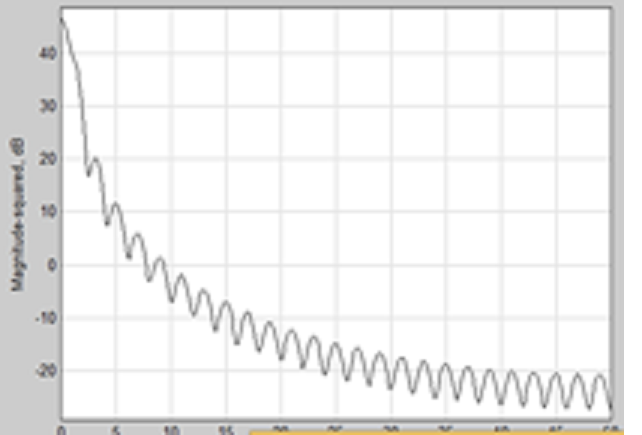
\includegraphics[angle=0, scale = 0.9]{5.png}\newline
рис. 5. спектр прямоугольного сигнала\newline
\end{center}
\end{figure}
\begin{figure}
\begin{center}
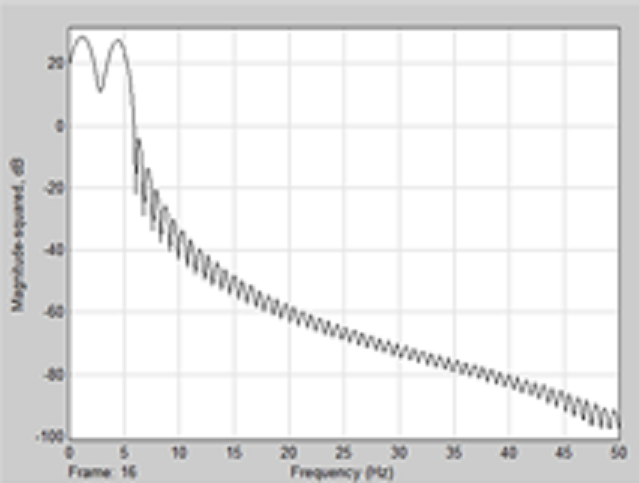
\includegraphics[angle=0, scale = 0.7]{6.png}\newline
рис. 6.спектр полигармонического сигнала\newline
\end{center}
\end{figure}
\begin{figure}
\begin{center}
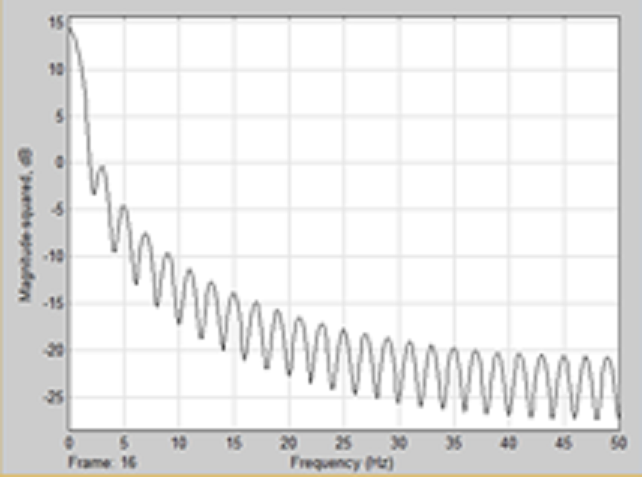
\includegraphics[angle=0, scale = 0.7]{7.png}\newline
рис. 7.спектр треугольного сигнала\newline
\end{center}
\end{figure}
\begin{figure}
\begin{center}
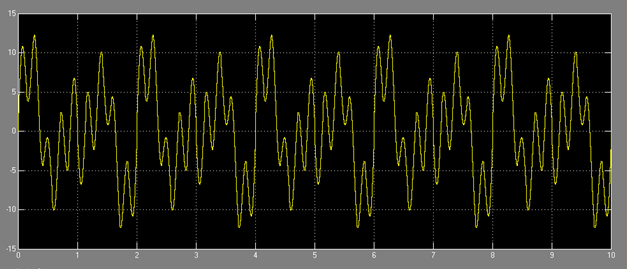
\includegraphics[angle=0, scale = 0.7]{8.png}\newline
рис. 8 полигармонический сигнал\newline
\end{center}
\end{figure}
\begin{figure}
\begin{center}
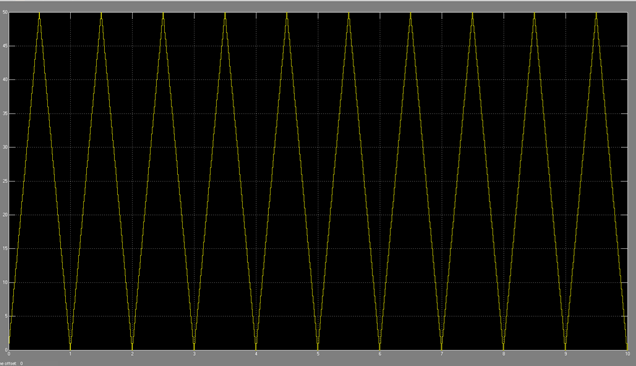
\includegraphics[angle=0, scale = 0.7]{9.png}\newline
рис. 9  треугольный сигнал\newline
\end{center}
\end{figure}
\begin{figure}
\begin{center}
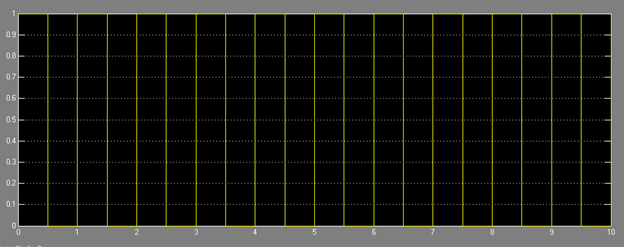
\includegraphics[angle=0, scale = 0.7]{10.png}\newline
рис. 10  прямоугольный сигнал\newline
\end{center}
\end{figure}


\begin{figure}
\begin{center}
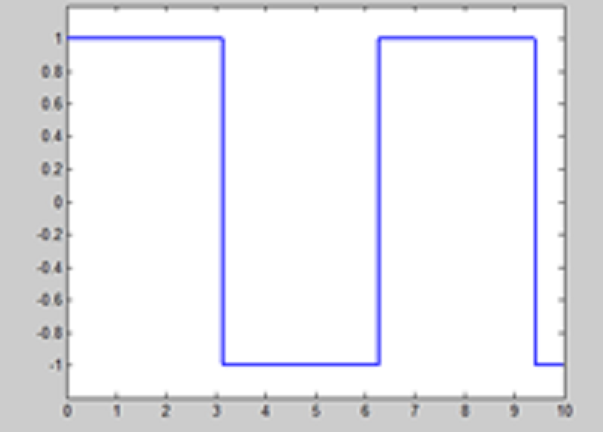
\includegraphics[angle=0, scale = 0.7]{11.png}\newline
рис. 11  прямоугольный сигнал\newline
\end{center}
\end{figure}

\begin{figure}
\begin{center}
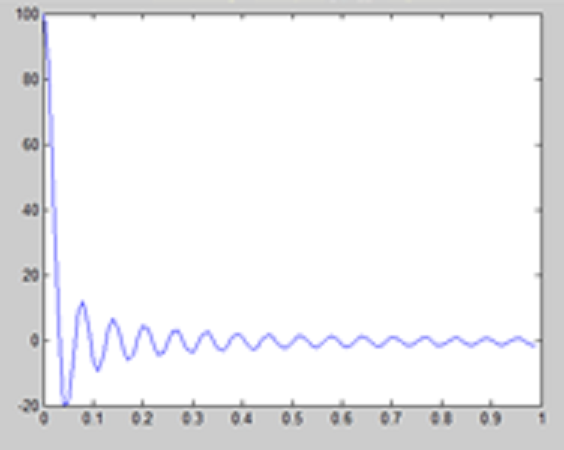
\includegraphics[angle=0, scale = 0.8]{12.png}\newline
рис. 12  полигармонический сигнал\newline
\end{center}
\end{figure}
\begin{figure}
\begin{center}
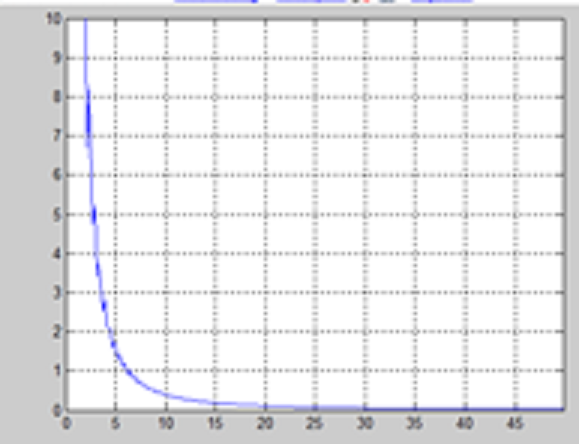
\includegraphics[angle=0, scale = 0.7]{13.png}\newline
рис. 13   спектр треугольного сигнала\newline
\end{center}
\end{figure}

\begin{figure}
\begin{center}
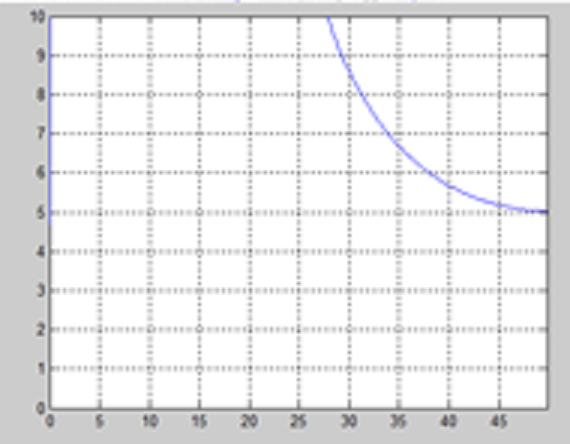
\includegraphics[angle=0, scale = 0.7]{14.png}\newline
рис. 14   спектр прямоугольного сигнала\newline
\end{center}
\end{figure}

\begin{figure}
\begin{center}
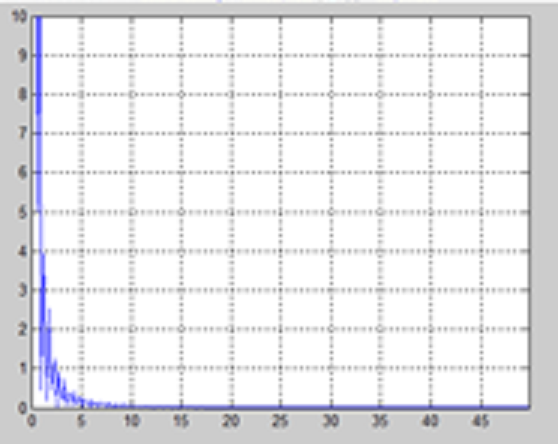
\includegraphics[angle=0, scale = 0.7]{15.png}\newline
рис. 15    спектр полигармонического сигнала\newline
\end{center}
\end{figure}

\begin{figure}
\begin{center}
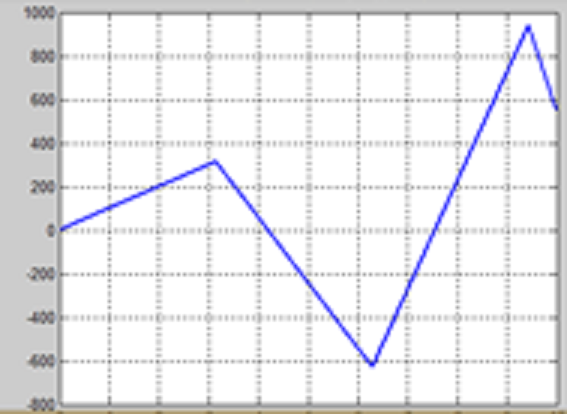
\includegraphics[angle=0, scale = 0.7]{16.png}\newline
рис. 16    треугольный сигнал\newline
\end{center}
\end{figure}


\clearpage
\section{Вывод}
В данной лабораторной работе было проведено моделирование полигармонического сигнала, прямоугольного сигнала и треугольного сигнала.
Были получены спектры данных сигналов. Для получения сигналов использовались математические формулы данных функций, а также средство моделирования Simulink. 
Обоими способами были получены спектры сигналов. Частным случаем в работе было получение треугольного сигнала через премение операции свертки над произведением 
двух прямоуголных сигналов. Данная операция осуществляется как математически, так и при моделировании в среде Simulink.
Обоснованием получения треугольного сигнала из свертки двух прямоугольных служит тот факт, что интеграл от произведения двух констант есть линейная функция. 
График такого преобразования будет представлять две линеных функции, одна из котрых имеет положительный коэффициента наклона, а другая отрицательный.

\chapter{Лабораторная работа №6. Линейная фильтрация}

\section{Теоретическая часть}
Фильтр низких частот - один из видов фильтров, эффективно пропускающий частотный спектр сигнала ниже определенной частоты (частоты среза) и уменьшающий частоты сигнала выше этой частоты. Для реализации фильтра в данной лабораторной работе был реализован фильтр Баттерворта. Фильтр Баттерворта проектируется так, чтобы его амплитудно-частотная характеристика была максимально гладкой на частотах полосы пропускания. Порядок фильтра прямопропорционален скорости подавления сигнала выше полосы пропускания. Так же замено, что при более высоком порядке фильтра, частота среза выражена ярче. Амплитудно-частотная характеристика G(w) фильтра Баттерворта n го порядка может быть получена из передаточной функции H(s):
\begin{displaymath}
	G^2(w) = |H^2(s)| = \frac{G_0^2}{1+(\frac{w}{w_c})^2}
\end{displaymath}
где:
\begin{itemize}
\item n — порядок фильтра
\item wc — частота среза (частота на которой амплитуда равна 3dB)
\item G0 — коэффициент усиления по постоянной составляющей (усиление на нулевой частоте)
\end{itemize}
\section{Алгоритм работы}
Сгенерировать гармонический сигнал с шумом и синтезировать ФНЧ. Получить сигнал во временной и частотной областях до и после фильтрации. Сделать выводы о воздействии ФНЧ на  спектр сигнала.
\section{Код MATLAB}
function seti6() \newline

x = 0:0.01:4*pi;\newline
f=100*(0:255)/512;\newline
figure(1)\newline
noise=rand(size(x));\newline
y = sin(2*pi*x);\newline
ynoisy = y+0.3*noise;\newline
plot(x(1:200),y(1:200))\newline
title('Исходный сигнал')\newline
grid\newline
figure(2)\newline
plot(x(1:200),ynoisy(1:200))\newline
title('Исходный сигнла с шумом')\newline
grid\newline
[B,A] = butter(16,0.98); % Синтез ФНЧ Баттерворта\newline
B=B./sum(B);\newline
A=A./sum(A);\newline
%Обработка сигнала ФНЧ\newline
figure(3)\newline
yfiltered = conv(ynoisy,[B,A]);\newline
plot(x(1:200),yfiltered(1:200))\newline
title('Отфильтрованный зашумленный сигнал')\newline
grid\newline
figure(4)\newline
normalspectrum = fft(y,512);\newline
normspectrum = normalspectrum.*conj(normalspectrum)/512;\newline
plot(f,normspectrum(1:256))\newline
axis([0 max(f) 0 2])\newline
title('Спектр исходного сигнала')\newline
grid\newline
figure(5)\newline
noisyspectrum = fft(ynoisy,512);\newline
normnoisyspectrum = noisyspectrum.*conj(noisyspectrum)/512;\newline
plot(f,normnoisyspectrum(1:256))\newline
axis([0 max(f) 0 2])\newline
title('Спектр зашумленного сигнала')\newline
grid\newline
figure(6)\newline
spectrum = fft(yfiltered,512);\newline
normfilteredspectrum=spectrum.*conj(spectrum)/512;\newline
plot(f,normfilteredspectrum(1:256))\newline
axis([0 max(f) 0 2])\newline
title('Спектр отфильтрованного сигнала')\newline
grid\newline
end\newline


\begin{figure}
\begin{center}
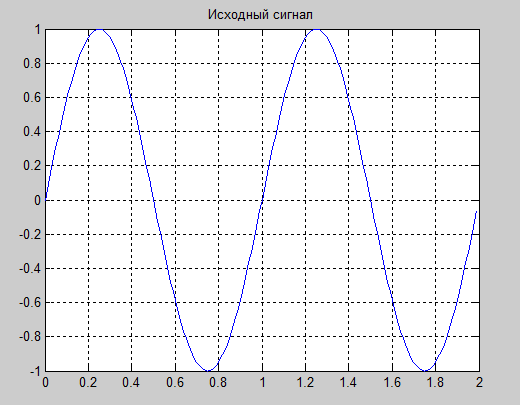
\includegraphics[angle=0, scale = 0.8]{6_1.png}\newline
рис.17. Исходный сигнал\newline
\end{center}
\end{figure}
\begin{figure}
\begin{center}
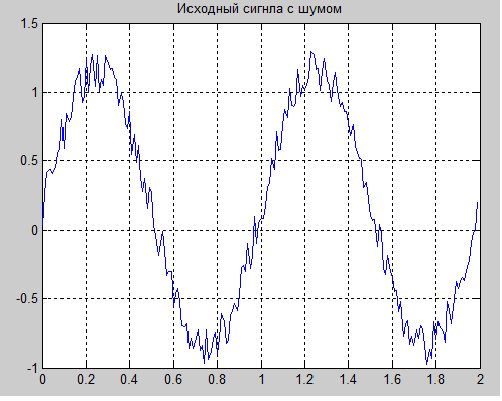
\includegraphics[angle=0, scale = 0.8]{6_2.png}\newline
рис.18. Зашумленный сигнал\newline
\end{center}
\end{figure}
\begin{figure}
\begin{center}
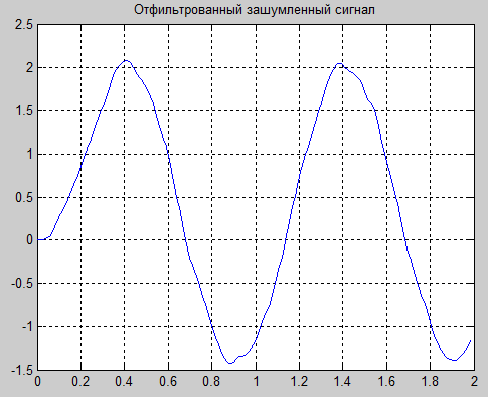
\includegraphics[angle=0, scale = 0.8]{6_3.png}\newline
рис.19. Отфильтрованный сигнал\newline
\end{center}
\end{figure}
\begin{figure}
\begin{center}
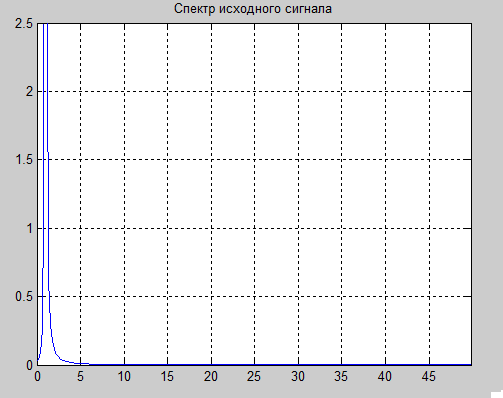
\includegraphics[angle=0, scale = 0.8]{6_4.png}\newline
рис.20. Спектр исходного сигнала\newline
\end{center}
\end{figure}
\begin{figure}
\begin{center}
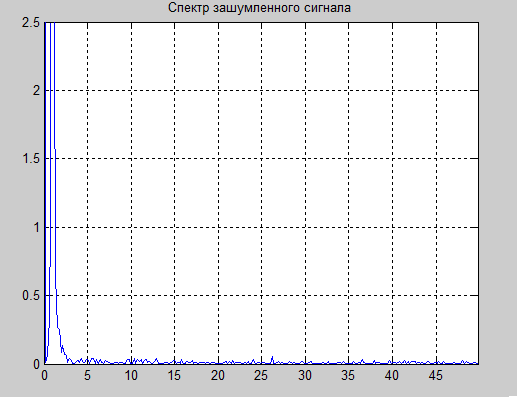
\includegraphics[angle=0, scale = 0.8]{6_5.png}\newline
рис.21. Спектр зашумленного сигнала\newline
\end{center}
\end{figure}
\begin{figure}
\begin{center}
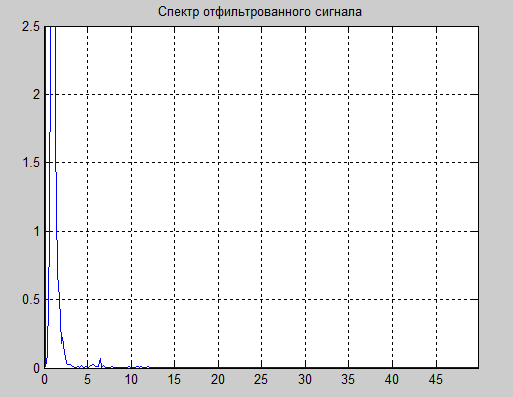
\includegraphics[angle=0, scale = 0.8]{6_6.png}\newline
рис.21. Спектр отфильтрованного сигнала\newline
\end{center}
\end{figure}
\clearpage
\section{Вывод}
В данной лабораторной работе был синтезирован фильтра Баттерворта 16 порядка и была исследована фильтрация зашумленного сигнала с помощью данного фильтра.
При фильтрации сигнала происходит подавление ненужных частот(частот шума), после чего сигнал приобретает форму, близкую к исходному. При этом фильтр
полностью не игнорирует все ненужные частоты в сигнале, это связано с наличием переходной зоны между частотами подавления сигнала и частотами пропускания сигнала.
Из-за наличия переходной зоны фильтра, он успевает захватить еще несколько частот. Для абсолютного подавления частот необходимо иметь иделаьный фильтр, который не имеет
переходной зоны между частотами подавления и пропускания. В результате использования такого фильтра будет происходить умножение исходного сигнала на прямоугольную функцию
в частотной области.


\chapter{Лабораторная работа №7. Аналоговая модуляция}
\section{Алгоритм работы}


	\begin{enumerate}
		\item Сгенерировать однотоальный сигнал низкой частоты.
		\item Выполнить амплитудную модуляцию сигнала по закону
				\begin{equation}
					u(t) = (1+MU_m cos(\Omega t))cos(\omega_0 t+\phi_0).
				\end{equation}
		\item Получить спектр модулированного сигнала.
		\item Выполнить модуляцию с подавлением несущей 
				\begin{equation}
					u(t) = MU_m cos(\omega t)cos(\omega_0 t+\phi_0).
				\end{equation}
		      Получить спектр. 
		\item Выполнить однополосную модуляцию:
				\begin{equation}
					u(t) = U_m cos(\omega t)cos(\omega_0 t+\phi_0)+\frac{U_m}{2}\sum_{n=1}^N M_n (cos(\omega_0 + \Omega_n )t + \phi_0 + \Phi_n ),
				\end{equation}
				положив n = 1.
		\item Выполить синхронное детектирование и получить исходный однополосный сигнал.
		\item Рассчитать КПД модуляции
				\begin{equation}
					\eta_A M = \frac{U_m ^2 M^2 /4}{P_U} = \frac{M^2}{M^2 + 2}.
				\end{equation}
	\end{enumerate}
\section{Код MATLAB}
function seti7() \newline
close all;\newline
x = 0:0.01:4*pi;\newline
f0 = 0.5;\newline

y = sin(2*pi*f0*x);\newline
figure(1)\newline
plot(x(1:1000),y(1:1000), 'LineWidth', 1)\newline
title('Однотональный сигнал низкой частоты')\newline
grid\newline

spectrum = fft(y, 1024);\newline
normspectrum = spectrum.*conj(spectrum)/1024;\newline
f = 100*(0:255)/1024;\newline
figure(2)\newline
plot(f, normspectrum(1:256), 'LineWidth', 1)\newline
axis([0 max(f) 0 150])\newline
title('Спектр исходного сигнала')\newline
grid\newline

Fc = 10*f0;\newline
Fs = 100*f0;\newline
U = ammod(y, Fc, Fs, 0, 1);\newline
figure(3)\newline
plot(x(1:1000), U(1:1000),  'LineWidth', 1)\newline
title('Модулированный сигнал')\newline
grid\newline

uspectrum = fft(U, 1024);\newline
normuspectrum = uspectrum.*conj(uspectrum)/1024;\newline
figure(4)\newline
plot(f, normuspectrum(1:256))\newline
axis([0 max(f) 0 70])\newline
title('Спектр модулированного сигнала')\newline
grid\newline

Fc = 10*f0;\newline
Fs = 100*f0;\newline
U = ammod(y, Fc, Fs);\newline
figure(5)\newline
plot(x(1:1000), U(1:1000), 'LineWidth', 1)\newline
title('Модуляция с подавлением несущей')\newline
grid\newline

uspectrum = fft(U, 1024);\newline
normuspectrum = uspectrum.*conj(uspectrum)/1024;\newline
figure(6)\newline
plot(f, normuspectrum(1:256))\newline
axis([0 max(f) 0 70])\newline
title('Спектр модулированного сигнала с подвалением несущей')\newline
grid\newline
\newline
Fc = 10*f0;\newline
Fs = 100*f0;\newline
U = ssbmod(y, Fc, Fs, [], 'upper');\newline
figure(7)\newline
plot(x(1:500), U(1:500), 'LineWidth', 1)\newline
title('Однополосая модуляция')\newline
grid\newline

uspectrum = fft(U, 1024);\newline
normuspectrum = uspectrum.*conj(uspectrum)/1024;\newline
figure(8)\newline
plot(f, normuspectrum(1:256))\newline
axis([0 max(f) 0 70])\newline
title('Спектр однополосной модуляции')\newline
grid\newline

[b, a] = butter(10, Fc*2/Fs);\newline
z = ssbdemod(U, Fc, Fs, 0, b, a);\newline
figure(9)\newline
plot(x(1:1000), z(1:1000), 'LineWidth', 1)\newline
title('Синхронное детектирование')\newline
grid\newline

duspectrum = fft(U, 1024);\newline
normduspectrum = duspectrum.*conj(duspectrum)/1024;\newline
figure(10)\newline
plot(f, normduspectrum(1:256))\newline
axis([0 max(f) 0 70])\newline
title('Спектр детектированного сигнала')\newline
grid\newline

M = 0.5;\newline
n = M*M/(M*M+2)\newline
end

\clearpage
\begin{figure}
\begin{center}
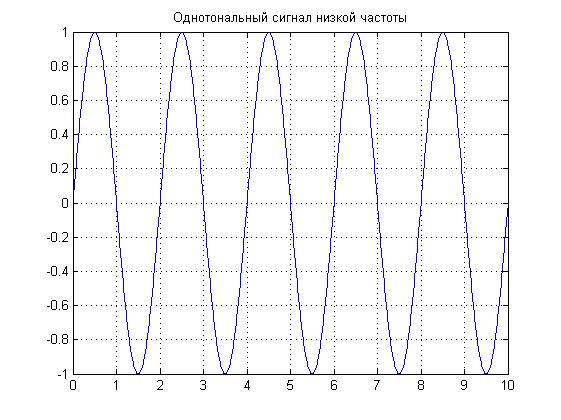
\includegraphics[angle=0, scale = 0.6]{7_1.jpg}\newline
рис. Исходный сигнал\newline
\end{center}
\end{figure}
\begin{figure}
\begin{center}
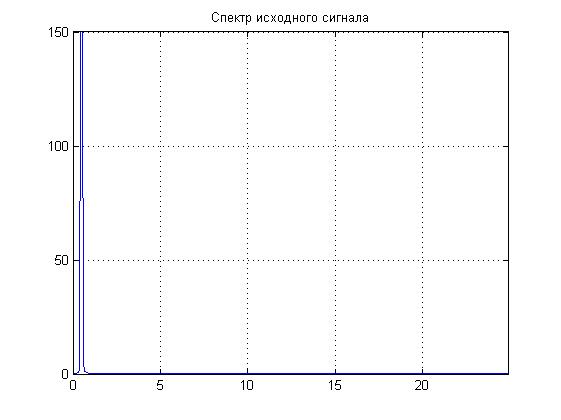
\includegraphics[angle=0, scale = 0.6]{7_2.jpg}\newline
рис. спектр исходного сигнала\newline
\end{center}
\end{figure}
\begin{figure}
\begin{center}
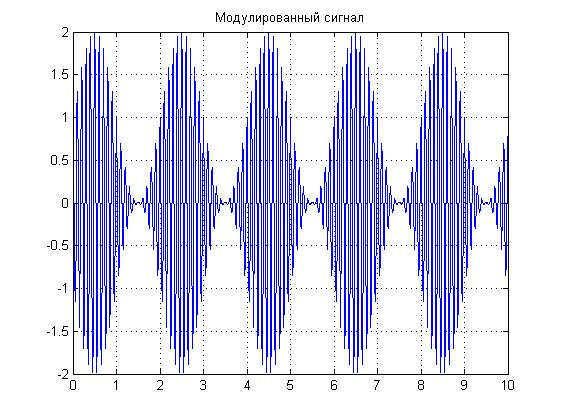
\includegraphics[angle=0, scale = 0.6]{7_3.jpg}\newline
рис. Модулированный сигнал\newline
\end{center}
\end{figure}
\begin{figure}
\begin{center}
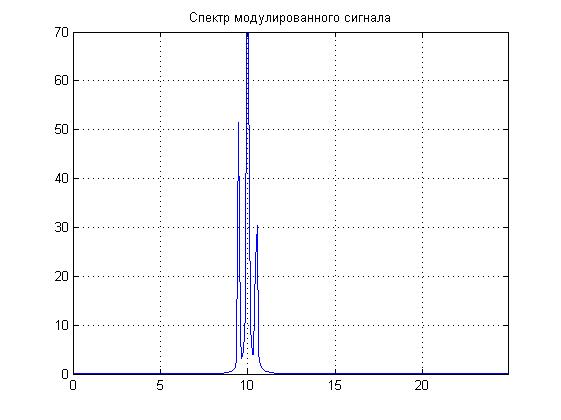
\includegraphics[angle=0, scale = 0.6]{7_4.jpg}\newline
рис. Спектр модулированного сигнала\newline
\end{center}
\end{figure}
\begin{figure}
\begin{center}
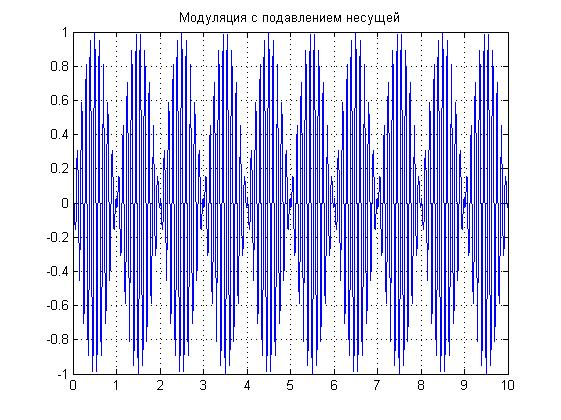
\includegraphics[angle=0, scale = 0.6]{7_5.jpg}\newline
рис. Сигнал с подавлением несущей\newline
\end{center}
\end{figure}
\begin{figure}
\begin{center}
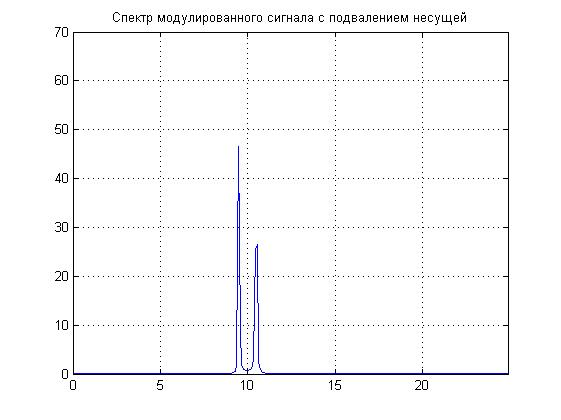
\includegraphics[angle=0, scale = 0.6]{7_6.jpg}\newline
рис. Спектр сигнала с подавлением несущей\newline
\end{center}
\end{figure}
\begin{figure}
\begin{center}
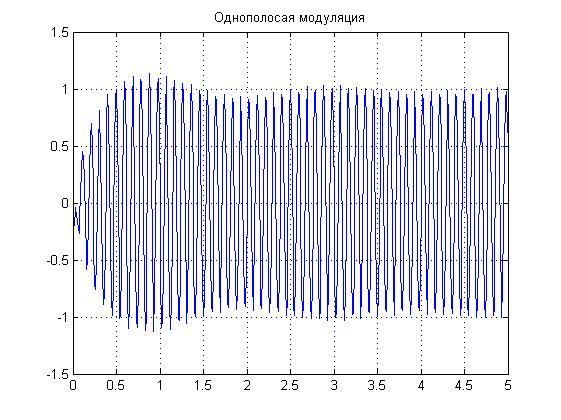
\includegraphics[angle=0, scale = 0.6]{7_7.jpg}\newline
рис. Однополосный сигнал\newline
\end{center}
\end{figure}
\begin{figure}
\begin{center}
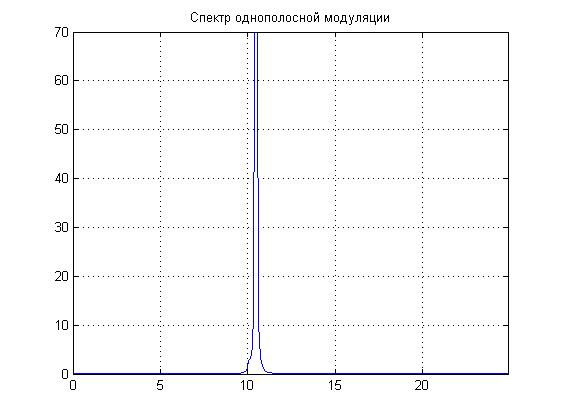
\includegraphics[angle=0, scale = 0.6]{7_8.jpg}\newline
рис. Спектр однополосного сигнала\newline
\end{center}
\end{figure}
\begin{figure}
\begin{center}
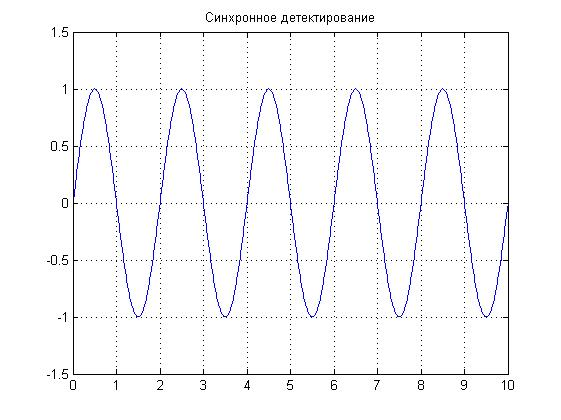
\includegraphics[angle=0, scale = 0.6]{7_9.jpg}\newline
рис.детектированный сигнал\newline
\end{center}
\end{figure}
\begin{figure}
\begin{center}
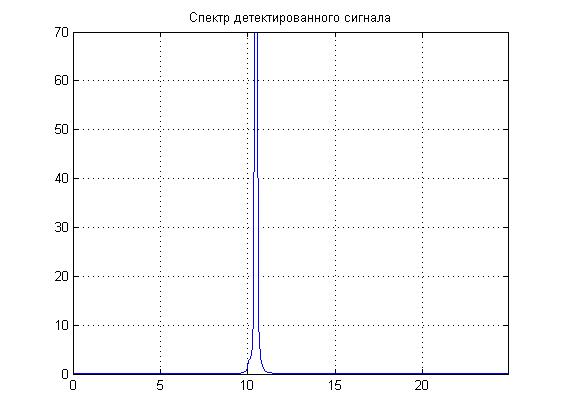
\includegraphics[angle=0, scale = 0.6]{7_10.jpg}\newline
рис. Спектр детектированного сигнала\newline
\end{center}
\end{figure}
\begin{figure}
\begin{center}
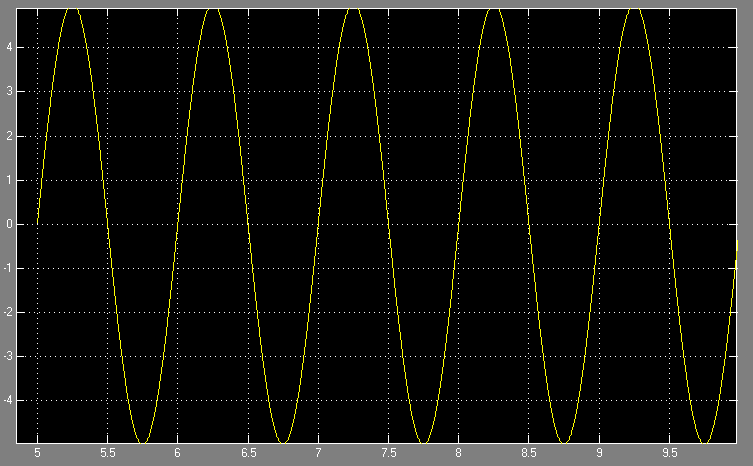
\includegraphics[angle=0, scale = 0.6]{7_11.png}\newline
рис. Исходный сигнал. Simulink\newline
\end{center}
\end{figure}
\begin{figure}
\begin{center}
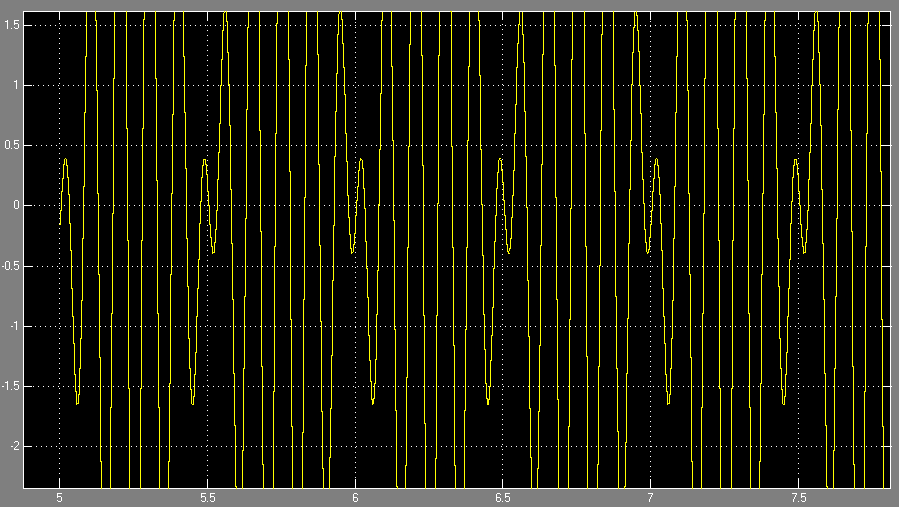
\includegraphics[angle=0, scale = 0.6]{7_12.png}\newline
рис.Модуляция Simulink\newline
\end{center}
\end{figure}
\begin{figure}
\begin{center}
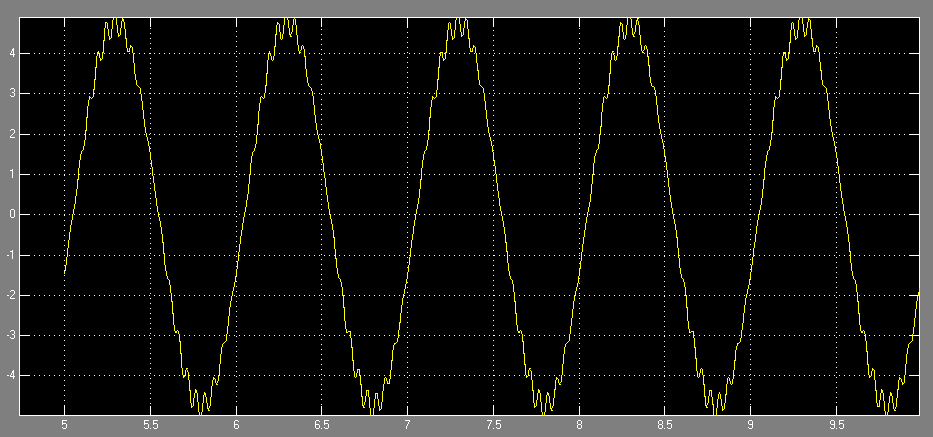
\includegraphics[angle=0, scale = 0.6]{7_13.png}\newline
рис.Демодуляция. Simulink\newline
\end{center}
\end{figure}
\begin{figure}
\begin{center}
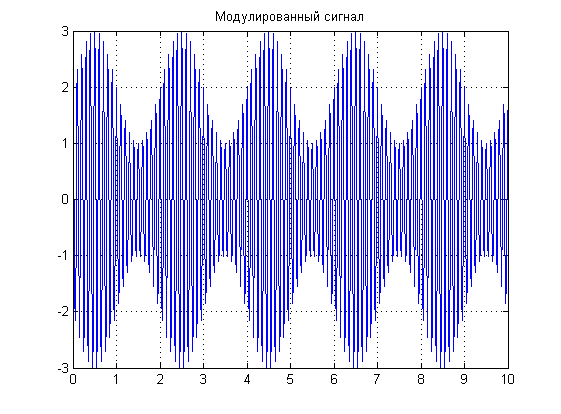
\includegraphics[angle=0, scale = 0.6]{7_14.png}\newline
рис. Модулированный сигнал с коэффициентом 2\newline
\end{center}
\end{figure}
\begin{figure}
\begin{center}
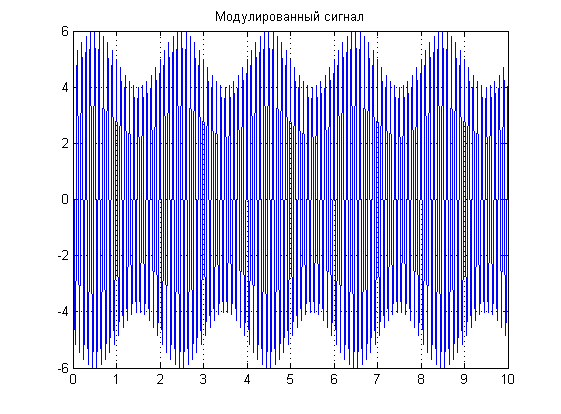
\includegraphics[angle=0, scale = 0.6]{7_15.png}\newline
рис. Модулированный сигнал с коэффициентом 5\newline
\end{center}
\end{figure}
\clearpage
\section{Вывод}
В данной лабораторной работе была исследована аналоговая модуляция. Был проведен эксперимент по изменению амплитуды сигнала.
Амплитудная модуляция применяется на низких частотах, что обусловлено низким КПД использования энергии модулированных сигналов.
Основным применением амплитудной модуляции является передача сигналов звуковой частоты. Для получения колебаний боковых частот без несущей применяют так называемую 
балансную модуляцию, основанную на том, что складывают два АМ колебания, у которых колебания боковых частот находятся в фазе, а несущих - в противофазе
 (или берут разность двух АМ колебаний, у которых боковые частоты в противофазе, а несущие - в фазе). КПД такой модуляции становится равно 100 процентам.
При этом спектр модулированного сигнала представляет собой три импульса, две из которых симметрично расположены относительно средней. Средний импульс обозначает 
спектр несущего сигнала.
В ходе работы была произведена модуляция с подавлением несущей.
При этом происходит игнорирование несущего сигнала, а источником информации являются два боковых сигнала. Спектр такого сигнала представляет собой два 
вертикальных симметричных импульса, что говорит об отсутствии несущего сигнала.
В работе была проведена модуляция однополосного сигнала. Данный сигнал используется для  уменьшения мошности потребления энергии для переноса информации и 
для осуществления переноса информации на более дальние расстояния. Спектры двух боковых полос АМ-сигнала являются зеркальным отражением друг друга, то есть они 
несут одну и ту же информацию. Поэтому одну из боковых полос можно удалить. Спектр такого сигнала представляет собой один импульс, так как в нем исключены несущий 
сигнал и половина исходного. 
Также было рассмотрено синхронное детектирование сигнала (демодуляция сигнала), в результате которого из модулированного 
сигнала был получен исходный сигнал. Суть детектирвоания состоит в умножении частоты сигнала на опорное колебание с несущей частотой. Результат умножения содержит 
два слагаемых: искомая амплитуда и АМ-сигнал с несущей частотой 2$\omega_0$, который легко удаляется путем пропускания сигнала через фильтр низких частот.
Спектр демодулированного сигнала отличается от первоначального. 
\chapter{Лабораторная работа №8}
\section{Постановка задачи}
\begin{enumerate}
\item 
Сгенерировать однотональный сигнал низкой частоты.
\item
Выполнитьфазовую модуляцию/демодуляцию сигнала по закону $u(t)=(U_m\cos(\omega t=ks(t))$ , используя встроенную функцию MatLab pmmod, pmdemod.
\item
Получить спектр модулированного сигнала.
\item
Выполнить частотную модуляцию/демодуляцию по закону 
\begin{equation}
u(t)=U_m\cos (\omega _0 t+k \int_0^t s(t)dt=\phi _0)
\end{equation}
используя встроенные функции Matlab fmmod, fmdemod.
\end{enumerate}
\section{Теоретическая часть}
Частотная модуляция — вид аналоговой модуляции, при котором информационный сигнал управляет частотой несущего колебания. По сравнению с амплитудной модуляцией здесь амплитуда остаётся постоянной.\newline
Фазовая модуляция — один из видов модуляции колебаний, при которой фаза несущего колебания управляется информационным сигналом. Фазомодулированный сигнал s(t) имеет следующий вид:
\begin{equation} 
s(t) = g(t) \sin[2 \pi f_c t + \varphi(t)] ,
\end{equation}
где $g(t)$ — огибающая сигнала; $\phi(t)$ является модулирующим сигналом; $f_c$ — частота несущего сигнала; t — время.\\
По характеристикам фазовая модуляция близка к частотной модуляции. В случае синусоидального модулирующего (информационного) сигнала, результаты частотной и фазовой модуляции совпадают.
\section{Код matlab}
\begin{verbatim}
x = 0:0.01:2;
u = cos(2*pi*x);

figure;
subplot(3,1,1);
plot(x,u);
grid;
am = fmmod(u,2,30,1);
subplot(3,1,2);
plot(x,am);
grid;
modulatedSpectr = fft(am,512);
normSpectrum = modulatedSpectr.*conj(modulatedSpectr)/512;
f = 100*(-256:255)/512;
subplot(3,1,3);
plot(f,normSpectrum);
grid;
axis([min(f) max(f) 0 max(normSpectrum)]);

figure;
subplot(3,1,1);
plot(x,u);
grid;
am = pmmod(u,5,1000,pi/2);
subplot(3,1,2);
plot(x,am);
grid;
modulatedSpectr = fft(am,512);
normSpectrum = modulatedSpectr.*conj(modulatedSpectr)/512;
f = 100*(-256:255)/512;
subplot(3,1,3);
plot(f,normSpectrum);
grid;
axis([min(f) max(f) 0 max(normSpectrum)]);
\end{verbatim}
\section{Результаты работы}
\begin{figure}
\begin{center}
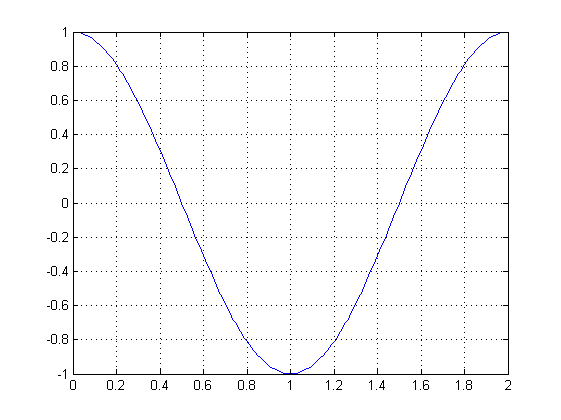
\includegraphics[angle=0, scale = 0.8]{8_1}\newline
рис. исходный сигнал\newline
\end{center}
\end{figure}
\begin{figure}
\begin{center}
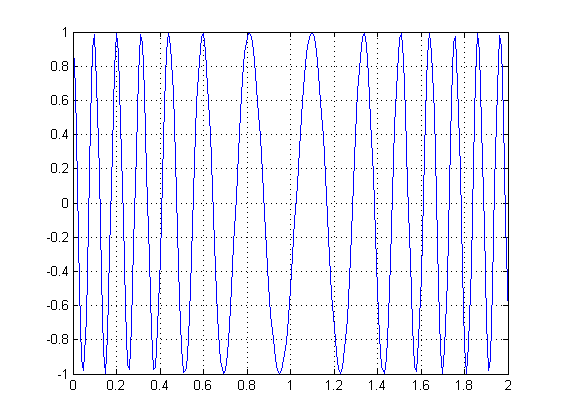
\includegraphics[angle=0, scale = 0.8]{8_2}\newline
рис. Частотная модуляция исходного сигнала\newline
\end{center}
\end{figure}
\begin{figure}
\begin{center}
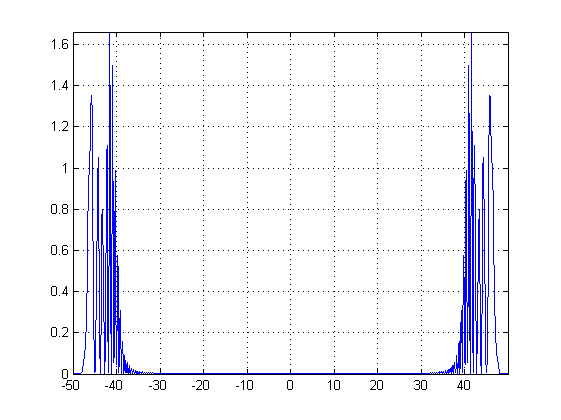
\includegraphics[angle=0, scale = 0.8]{8_3}\newline
рис.  Спектр частотной модуляции\newline
\end{center}
\end{figure}
\begin{figure}
\begin{center}
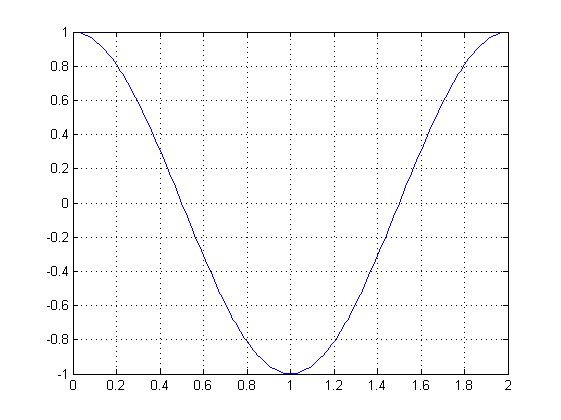
\includegraphics[angle=0, scale = 0.8]{8_4}\newline
рис. Исходный сигнал\newline
\end{center}
\end{figure}
\begin{figure}
\begin{center}
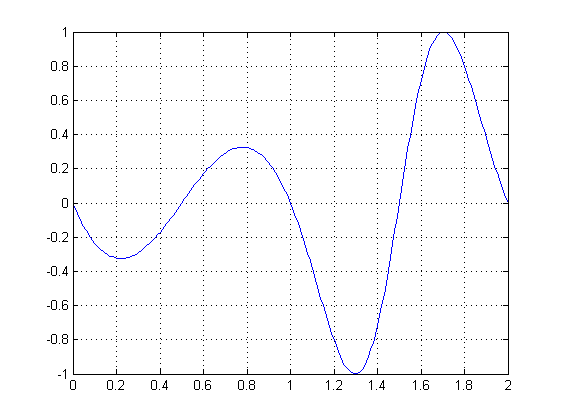
\includegraphics[angle=0, scale = 0.8]{8_5}\newline
рис.Фазовая модуляция\newline
\end{center}
\end{figure}
\begin{figure}
\begin{center}
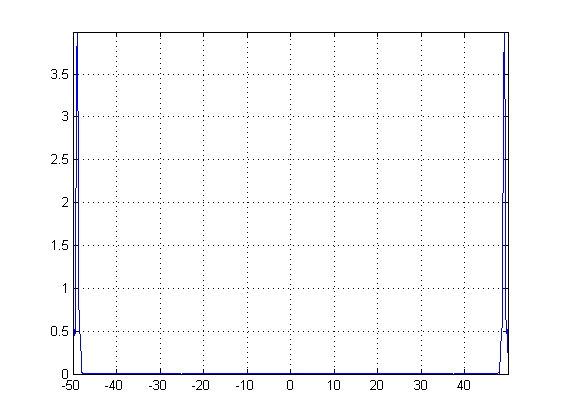
\includegraphics[angle=0, scale = 0.8]{8_6}\newline
рис. Спектр фазовой модуляции\newline
\end{center}
\end{figure}

\begin{figure}
\begin{center}
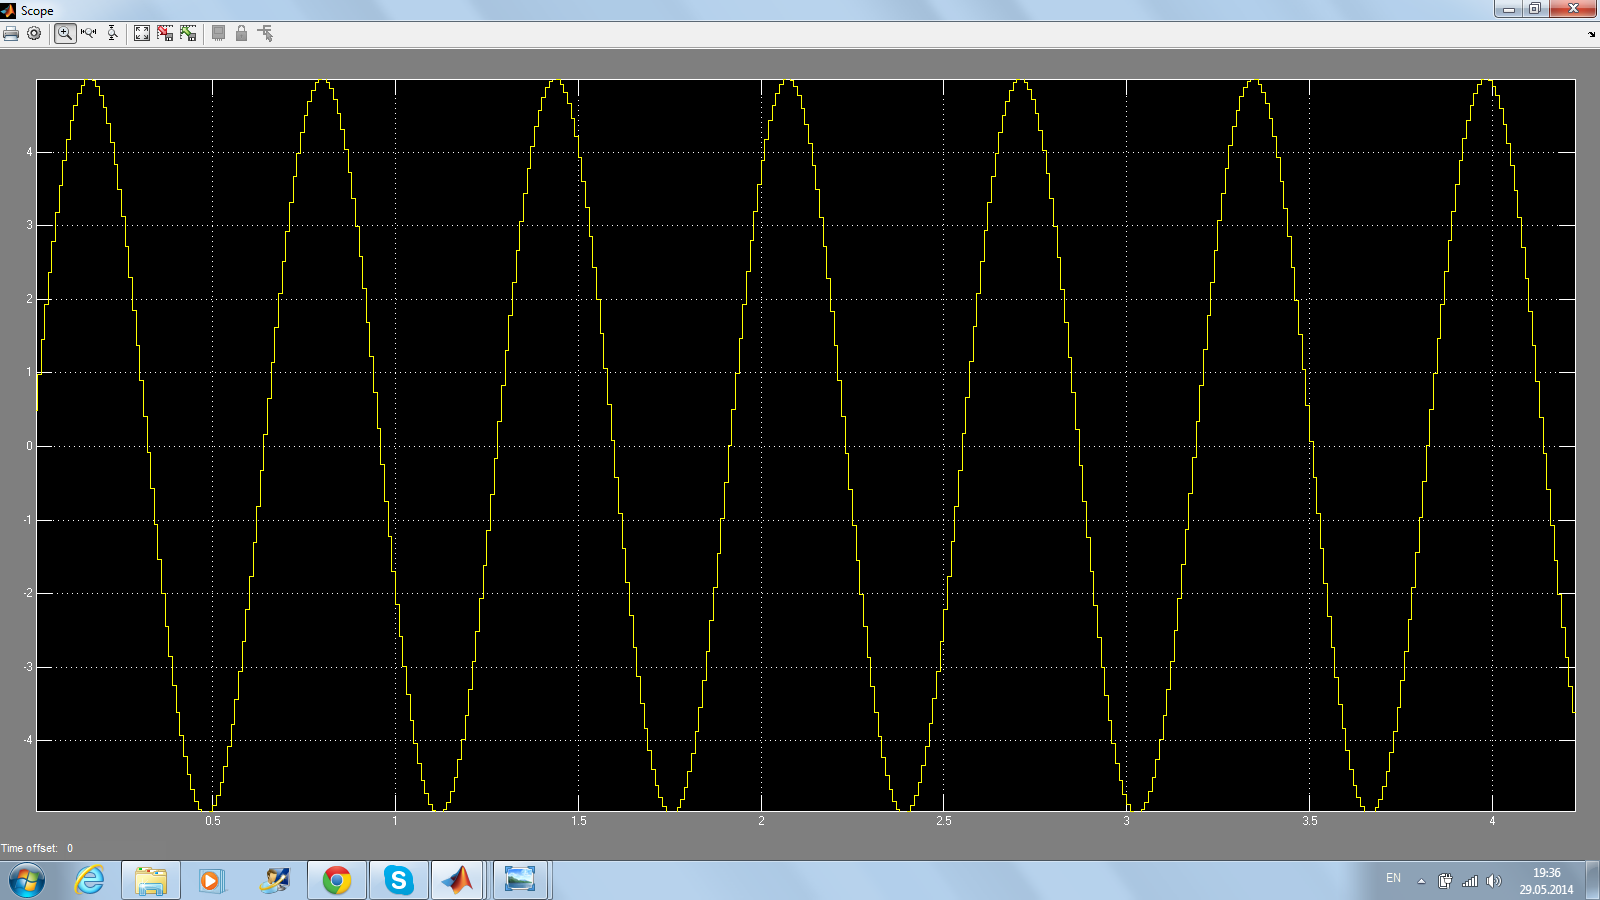
\includegraphics[width=150mm, scale = 0.9]{8_8}\newline
рис. Симулинк исходный сигнал\newline
\end{center}
\end{figure}
\begin{figure}
\begin{center}
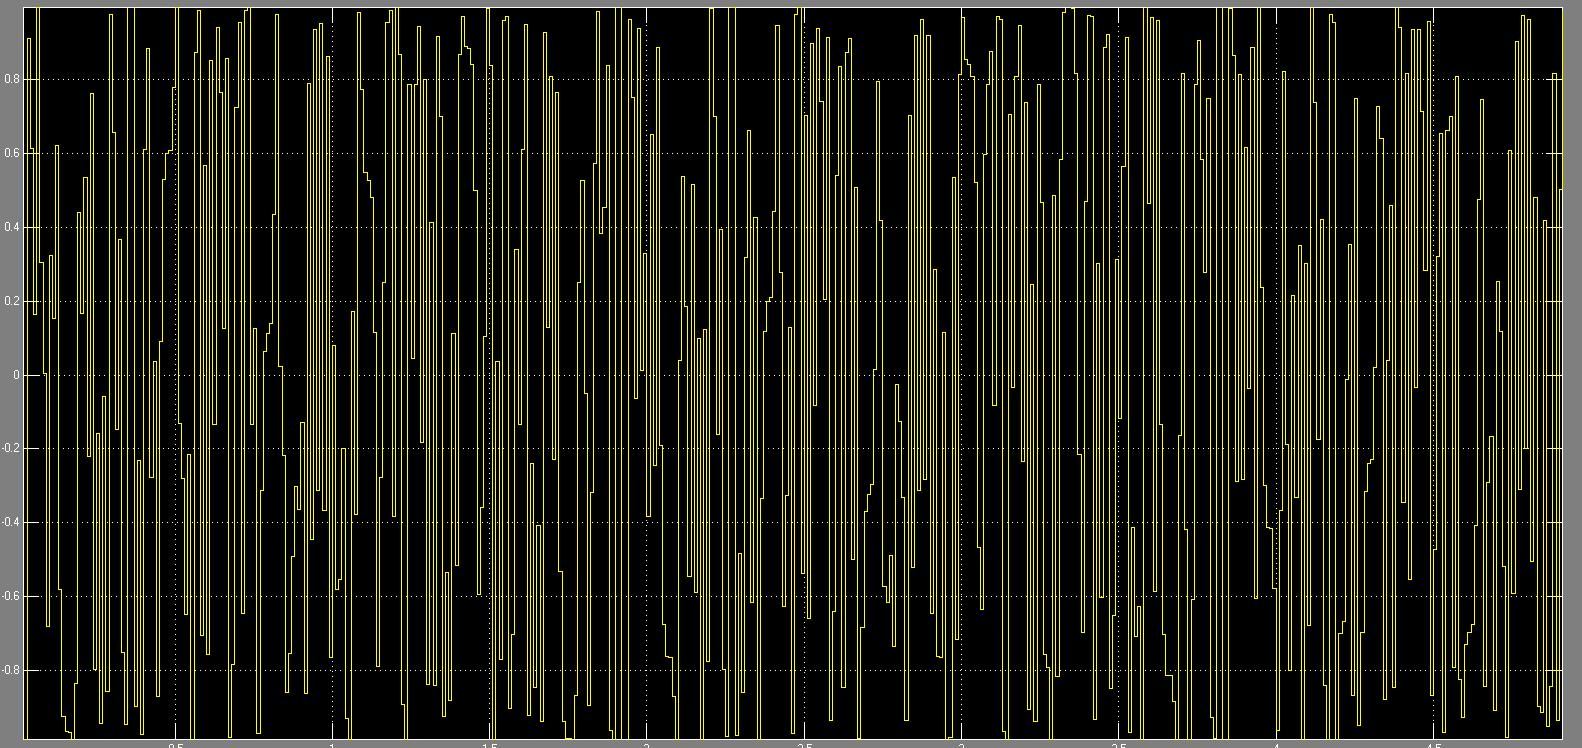
\includegraphics[width=150mm, scale = 0.9]{8_9}\newline
рис .Симулинк частотная модуляция\newline
\end{center}
\end{figure}
\begin{figure}
\begin{center}
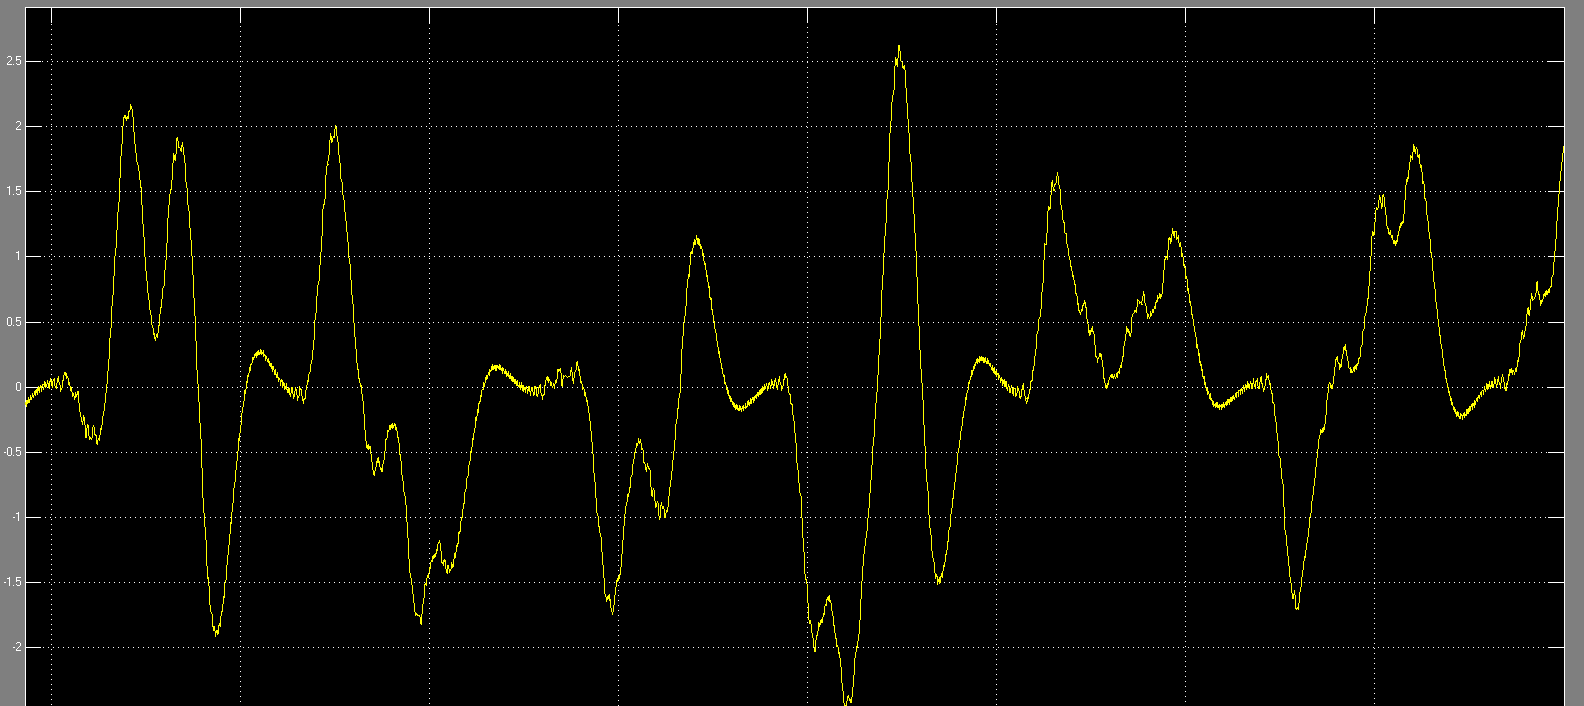
\includegraphics[width=150mm, scale = 0.9]{8_10}\newline
рис. Симулинк сигнал на выходе ФНЧ\newline
\end{center}
\end{figure}
Выполним демодуляцию, в том числе с помощью блока захвата фазы (фазовой автоподстройки частоты) Phase-Locked Loop.
\begin{figure}
\begin{center}
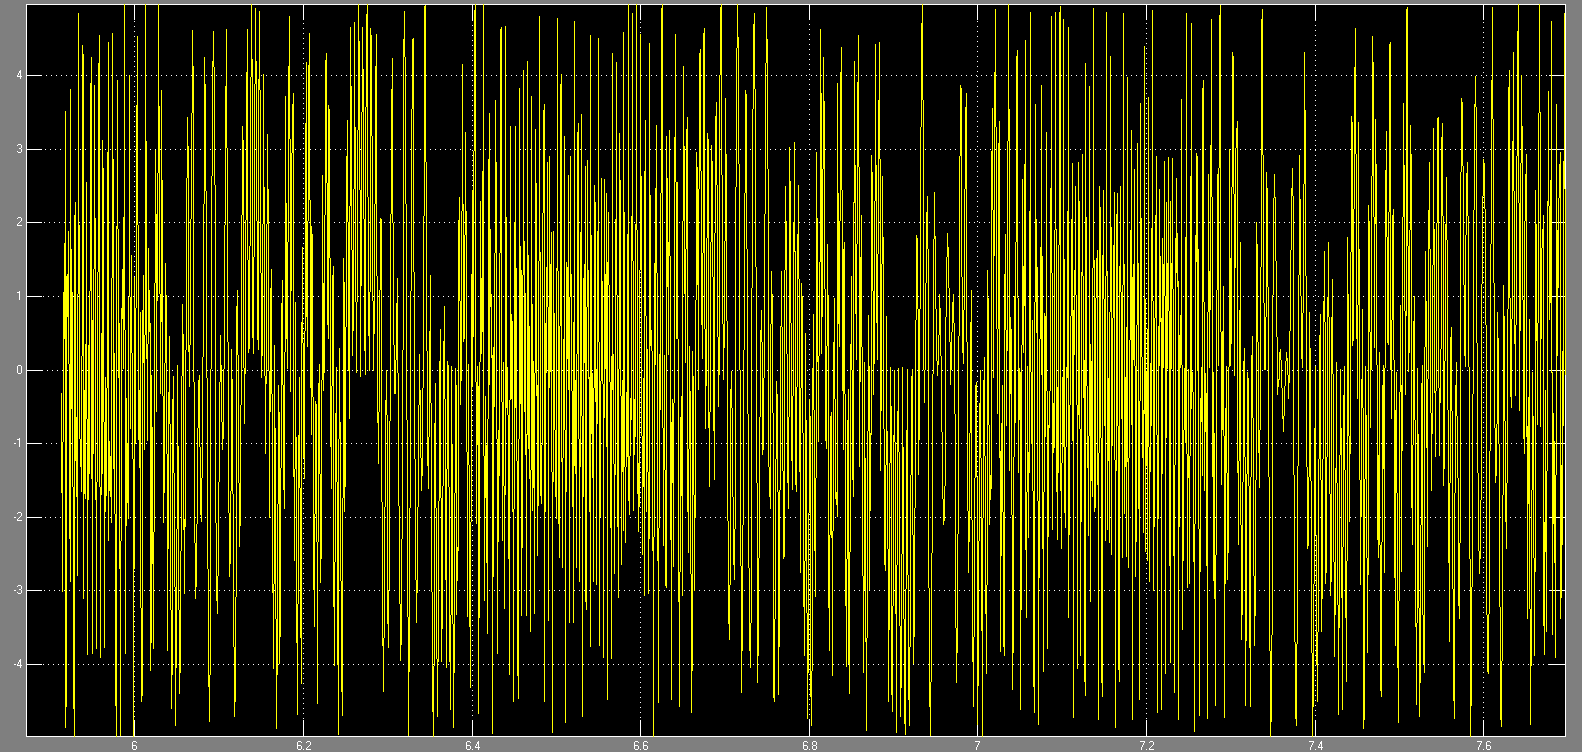
\includegraphics[width=150mm, scale = 0.9]{8_11}\newline
рис. Частотная модуляция PLL\newline
\end{center}
\end{figure}
\begin{figure}
\begin{center}
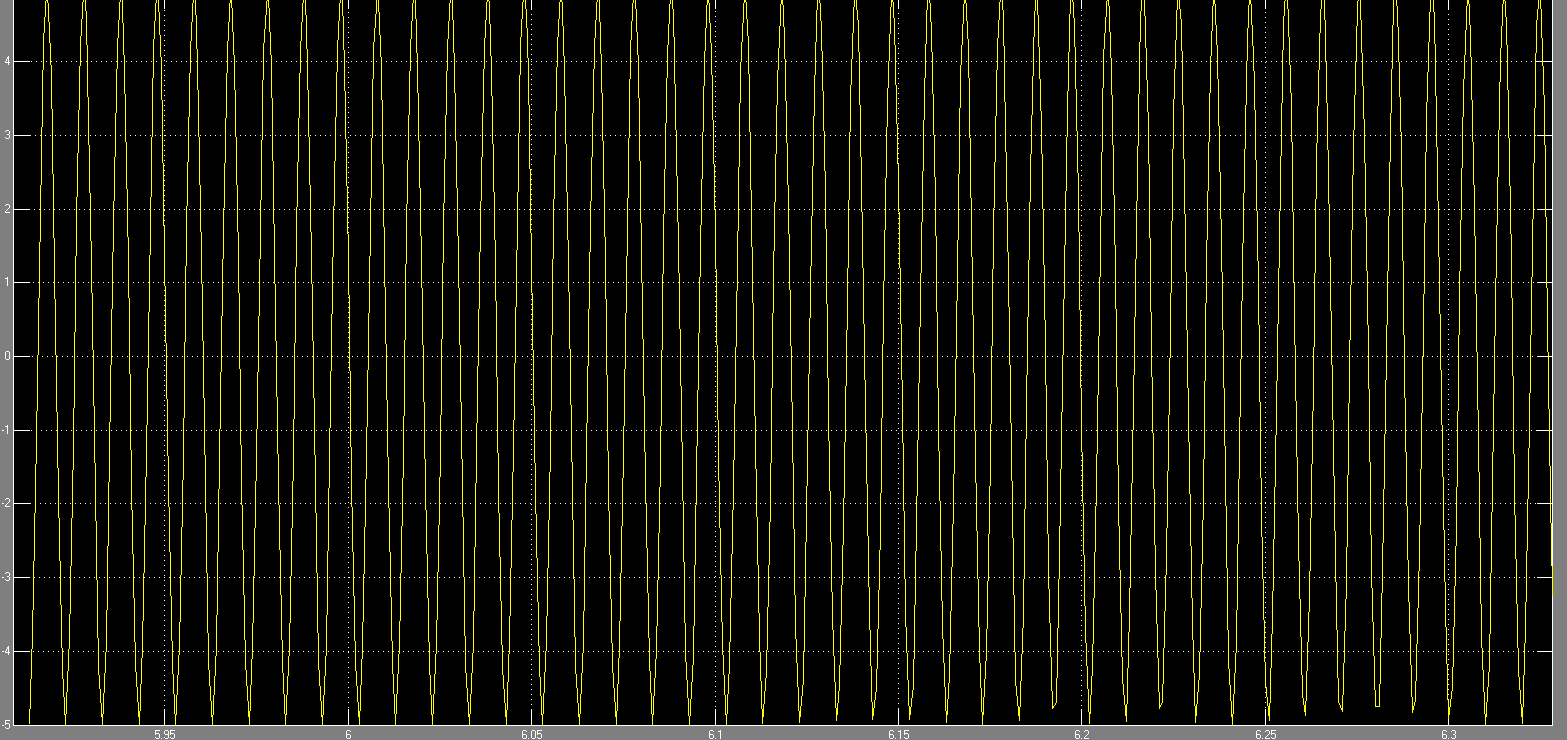
\includegraphics[width=150mm, scale = 0.7]{8_12}\newline
рис. Сигнал на выходе фазового детектора\newline
\end{center}
\end{figure}
\begin{figure}
\begin{center}
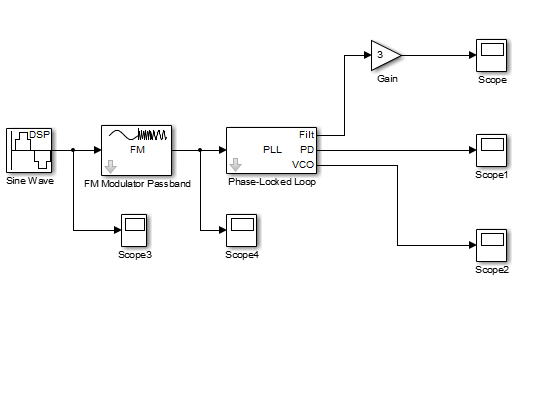
\includegraphics[width=150mm, scale = 0.7]{8_13}\newline
рис. Схема симулинк\newline
\end{center}
\end{figure}

\clearpage
\section{Вывод}
В данной лабораторной работе было проведено исследование частотной и фазовой модуляций/демодуляций. Частотная модуляция представляет собой изменение частоты исходного сигнала
при постоянной фазе и амплитуде. При этом происходит изменением длины волн сигнала на разных временных промежутках. Фазовая модуляция представляет собой изменение исходного
сигнала по фазе при постоянной амплитуде и постоянной частоте. При фазовой модуляции происходит изменение формы сигнала на отдельных промежутках. Фазовая и частотная модуляции
позволяют производить передачу высокочастотного звукового сигнала. Спектр частной модуляции представляет собой несколько вертикальных импульсов расположенных относительно центра 
спектральной прямой, это говорит о наличии нескольких гармониках в сигнале. Спектр фазовой модуляции представляет собой также несколько импульсов расположенных симметрично 
относительно центра спектральной прямой.Различие между фазовой и частотной модуляцией обнаруживается при модуляции спектром частот. При фазовой модуляции индекс модуляции 
(отношение девиации фазы к фаземодулирующего сигнала) не зависит от частоты модуляции, а девиация частоты (амплитуда изменения частоты) пропорциональна частоте модуляции. При частотной модуляции 
девиация частоты не зависит от частоты модуляции, а индекс модуляции (отношение девиации частоты к частоте модулирующего сигнала) обратно пропорционален частоте модуляции.
Частотную и фазовую модуляцию объединяют под общим названием угловой модуляции (УМ). По форме колебаний с угловой модуляцией невозможно определить, к какому виду модуляции 
относится данное колебание, к ФМ или ЧМ, а при достаточно гладких функциях формы сигналов ФМ и ЧМ вообще практически не отличаются. 
Также в лабораторной работе произведена частотная модуляции с использованием устройства фазовой автоподстройки частоты.Данное устройство представляет собой систему 
автоматического регулиярования, подстраивающая фазу управляемого генератора так, чтобы она была равна фазе опорного сигнала, либо отличалась на известную функцию от времени. 
Регулировка осуществляется благодаря наличию отрицательной обратной связи. Данный прибор используется для частотной модуляции и демодуляции, преобразования частоты и 
частотной фильтрации. 

\chapter{Лабораторная работа №9}
\section{Постановка задачи}
\begin{enumerate}
\item 
Получить сигналы BPSK, PSK, OQPSK, genQAM, MSK, M-FSK модуляторов.
\item
Построить их сигналы
\item
Провестисравнение изученных методов модуляции цифровых сигналов.
\end{enumerate}
\section{Теоретическая часть}
Сущность цифровой модуляции заключается в том, что передаваемый непрерывный сигнал дискретизируется во времени, квантуется по уровню и полученные отчеты, следующие в дискретные моменты времени, преобразуются в кодовые комбинации. Полученной последовательностью кодовых видеосигналов модулируется высокочастотный сигнал-переносчик.
Существует 3 основных вида манипуляции сигналов: амплитудная (Amplitude-shift keying (ASK)), частотная (Frequency-shift keying (FSK)) и фазовая (Phase-shift keying (PSK)). Этот набор манипуляций определяется основными характеристиками, которыми обладает любой сигнал. Для моделирования модуляции цифрового сигнала в ходе лаботаторной работы предлагается использовать следующий набор функций:
\begin{enumerate}
\item Функция randerr предназначена для формирования ошибок в цифровом сигнале. Она дает матрицу, в каждой строке которой имеется заданное число случайно расположенных ненулевых элементов.
\item Для оценки помехоустойчивости системы связи необходимо произвести сравнение исходного (передаваемого) сообщения с сообщением, полученным в результате приема, и определить число ошибок, возникших в процессе передачи, а также вероятность ошибки. Эти действия выполняются функциями symerr и biterr, первая из которых подсчитывает число несовпадающих символах в двух сообщениях, а вторая — число несовпадающих битов в двоичных представлениях этих символов. Кроме числа ошибок, обе функции могут возвращать долю ошибок в общем числе символов (битов) и индикаторы мест возникновения ошибок.
\item Последние две функции данной группы предназначены для графического отображения сигналов с квадратурной манипуляцией. Функция eyediagram выводит так называемую глазковую диаграмму, а функция scatterplot — диаграмму рассеяния.
\end{enumerate}
\begin{enumerate}
\item Амплитудная манипуляция (ASK) — изменение сигнала, при котором скачкообразно меняется амплитуда несущего колебания. АМн можно рассматривать как частный случай квадратурной манипуляции.
\item При частотной манипуляции (FSK) значениям «0» и «1» информационной последовательности соответствуют определённые частоты синусоидального сигнала при неизменной амплитуде. Частотная манипуляция весьма помехоустойчива. Однако при частотной манипуляции неэкономно расходуется ресурс полосы частот телефонного канала. Поэтому этот вид модуляции применяется в низкоскоростных протоколах, позволяющих осуществлять связь по каналам с низким отношением сигнал/шум.
\item Минимальная частотная модуляция (MSK) представляет собой способ модуляции, при котором не происходит скачков фазы и изменение частоты происходит в моменты пересечения несущей нулевого уровня. MSK уникальна потому, что значение частот соответствующих логическим «0» и «1» отличаются на величину равную половине скорости передачи данных.
\item Фазовая манипуляция (PSK) — один из видов фазовой модуляции, при которой фаза несущего колебания меняется скачкообразно в зависимости от информационного сообщения.
\item Квадратурной амплитудной манипуляцией (QASK) называется манипуляция, при которой изменяется как фаза, так и амплитуда сигнала, что позволяет увеличить количество информации, передаваемой одним состоянием (отсчётом) сигнала. 
\end{enumerate}
\section{Код matlab}
\begin{verbatim}
%BPSK modulation
h = modem.pskmod('M', 2);
g = modem.pskdemod('M', 2);
msg = randint(10,1,2);
modSignal = modulate(h,msg);
errSignal = (randerr(1,10, 3) ./ 30)';
modSignal = modSignal + errSignal;
demodSignal = demodulate(g,modSignal);
scatterplot(modSignal);
eyediagram(modSignal,10);
scatterplot(demodSignal);
eyediagram(demodSignal,10);

%PSK modulation
h = modem.pskmod('M', 8);
g = modem.pskdemod('M', 8);
msg = randint(10,1,8);
modSignal = modulate(h,msg);
errSignal = (randerr(1,10, 3) ./ 30)';
modSignal = modSignal + errSignal;
demodSignal = demodulate(g,modSignal);
scatterplot(modSignal);
eyediagram(modSignal,10);
scatterplot(demodSignal);
eyediagram(demodSignal,10);

%OQPSK modulation
h = modem.oqpskmod;
g = modem.oqpskdemod;
msg = randint(200,1,4);
modSignal = modulate(h,msg);
errSignal = (randerr(1,400, 100) ./ 30)';
modSignal = modSignal + errSignal;
demodSignal = demodulate(g,modSignal);
scatterplot(modSignal);
eyediagram(modSignal,10);
scatterplot(demodSignal);
eyediagram(demodSignal,10);

%GENQAM modulation
M = 5;
h = modem.genqammod('Constellation', exp(1i*2*pi*[0:M-1]/M));
g = modem.genqamdemod('Constellation', exp(1i*2*pi*[0:M-1]/M));
msg = randint(10,1,8);
modSignal = modulate(h,msg);
errSignal = (randerr(1,10, 3) ./ 30)';
modSignal = modSignal + errSignal;
demodSignal = demodulate(g,modSignal);
scatterplot(modSignal);
eyediagram(modSignal,10);
scatterplot(demodSignal);
eyediagram(demodSignal,10);

%MSK modulation
h = modem.mskmod('SamplesPerSymbol', 10);
g = modem.mskdemod('SamplesPerSymbol', 10);
msg = randint(10,1,2);
modSignal = modulate(h, msg);
errSignal = (randerr(1,100, 3) ./ 30)';
modSignal = modSignal + errSignal;
demodSignal = demodulate(g, modSignal);
scatterplot(modSignal);
eyediagram(modSignal,10);
scatterplot(demodSignal);
eyediagram(demodSignal,10);
\end{verbatim}
\section{Результаты работы}
\clearpage
\begin{figure}
\begin{center}
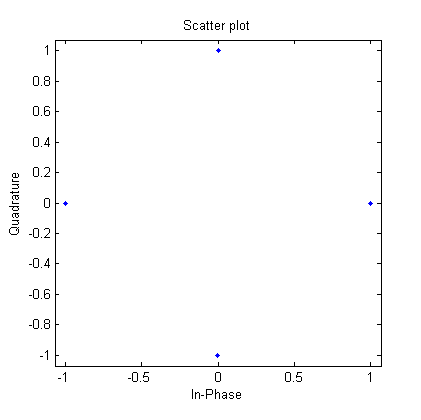
\includegraphics[angle=0, scale = 0.8]{9_1}\newline
рис. Сигнальное создвездие BPSK-модуляции\newline
\end{center}
\end{figure}
\begin{figure}
\begin{center}
\includegraphics[angle=0, scale = 0.8]{9_2}\newline
рис. Сигнальное созвездие BPSK-демодуляции\newline
\end{center}
\end{figure}
\begin{figure}
\begin{center}
\includegraphics[angle=0, scale = 0.8]{9_3}\newline
рис.Сигнальное созвездие PSK-модуляции\newline
\end{center}
\end{figure}
\begin{figure}
\begin{center}
\includegraphics[angle=0, scale = 0.8]{9_4}\newline
рис. Сигнальное созвездие PSK-демодуляции\newline
\end{center}
\end{figure}
\begin{figure}
\begin{center}
\includegraphics[angle=0, scale = 0.8]{9_5}\newline
рис.  Сигнальное созвездие OQPSK-модуляции\newline
\end{center}
\end{figure}
\begin{figure}
\begin{center}
\includegraphics[angle=0, scale = 0.8]{9_6}\newline
рис.  Сигнальное созвездие OQPSK-демодуляции\newline
\end{center}
\end{figure}
\begin{figure}
\begin{center}
\includegraphics[angle=0, scale = 0.8]{9_7}\newline
рис.  Сигнальное созвездие GENQAM-модуляции\newline
\end{center}
\end{figure}
\begin{figure}
\begin{center}
\includegraphics[angle=0, scale = 0.8]{9_8}\newline
рис. Сигнальное созвездие GENQAM-демодуляции\newline
\end{center}
\end{figure}
\begin{figure}
\begin{center}
\includegraphics[angle=0, scale = 0.8]{9_9}\newline
рис.  Сигнальное созвездие MSK-модуляции\newline
\end{center}
\end{figure}
\begin{figure}
\begin{center}
\includegraphics[angle=0, scale = 0.8]{9_10}\newline
рис. Сигнальное созвездие MSK-демодуляции\newline
\end{center}
\end{figure}

\begin{figure}
\begin{center}
\includegraphics[width=150mm, scale = 0.9]{9_21}\newline
рис. 85. Модель BPSK-модуляции\newline
\end{center}
\end{figure}


\begin{figure}
\begin{center}
\includegraphics[width=150mm, scale = 0.9]{9_22}\newline
рис. 86. Сигнальное созвездие BPSK-модуляции\newline
\end{center}
\end{figure}
\begin{figure}
\begin{center}
\includegraphics[width=150mm, scale = 0.9]{9_23}\newline
рис. 87. Модель PSK-модуляции\newline
\end{center}
\end{figure}
\begin{figure}
\begin{center}
\includegraphics[width=150mm, scale = 0.9]{9_24}\newline
рис. 88. Сигнальное созвездие PSK-модуляции.\newline
\end{center}
\end{figure}
\begin{figure}
\begin{center}
\includegraphics[width=150mm, scale = 0.9]{9_25}\newline
рис. 89. Модель OQPSK-модуляции\newline
\end{center}
\end{figure}

\begin{figure}
\begin{center}
\includegraphics[width=150mm, scale = 0.9]{9_26}\newline
рис. 90. Сигнальное созвездие OQPSK-модуляции.\newline
\end{center}
\end{figure}
\begin{figure}
\begin{center}
\includegraphics[width=150mm, scale = 0.9]{9_27}\newline
рис. 91. Модель genQAM-модуляции\newline
\end{center}
\end{figure}

\begin{figure}
\begin{center}
\includegraphics[width=150mm, scale = 0.9]{9_28}\newline
рис. Сигнальное созвездие genQAM-модуляции\newline
\end{center}
\end{figure}
\clearpage
\begin{figure}
\begin{center}
\includegraphics[width=150mm, scale = 0.9]{9_29}\newline
рис. Модель MSK-модуляции\newline
\end{center}
\end{figure}

\begin{figure}
\begin{center}
\includegraphics[width=150mm, scale = 0.9]{9_30}\newline
рис.  Сигнальное созвездие MSK-модуляции\newline
\end{center}
\end{figure}
\clearpage
\section{Вывод}
В данной лабораторной работе было проведено исследование цифровой модуляции для различных модуляторов: BPSK, PSK, OQPSK, GENQAM, MSK.Для каждого способа цифровой модуляции
были получены сигнальные созвездия модуляции и демодуляции. Радиосигнал представляется в виде двухмерной точечной диаграммы на комплексной плоскости, точками на которой 
являются все возможные символы, представленные в геометрической форме. Более абстрактно, на диаграмме отмечены все значения, которые могут быть выбраны данной схемой 
манипуляции, как точки на комплексной плоскости. Сигнальные созвездия, полученные в результате измерения радиосигнала, могут использоваться для определения типа манипуляции
 и уровня искажений.При представлении передаваемого символа в виде комплексного числа и при модуляции косинусного и синусного сигналов несущей частоты, 
соответственно действительной и мнимой частями, символ можно передать двумя несущими с одной частотой. Часто такие несущие называются квадратурными.
 Если символы представлены в виде комплексных чисел, их можно представить в виде точек на комплексной плоскости. Действительная и мнимая оси часто называют in phase (синфазной)
 или I-осью и quadrature (квадратурной) или Q-осью. При нанесении на диаграмму точек от нескольких символов можно получить сигнальное созвездие. Точки созвездия
 представляют множество модулирующих символов, то есть модулирующий алфавит.
При сравнении методов модуляции видно, что все созвездия, кроме случая с OQPSK модулятором, наносятся на круг с центром в начале координат и определенного радиуса. При осуществлении модуляции каждого типа 
количество точек в каждом типе модуляции увеличивается. При демодуляции точки налагают на ось абцисс координат.
Результат сравнения ошибок всех типов модуляции:
BPSK - 0; PSK - 0; OQPSK - 74; MSK - 0; M-FSK - 50 - Число несовпадающих символов в двух сообщениях (разница между символами исходного сигнала и демодулированного).
Уровень модуляции определяет количество состояний несущей, используемых для передачи информации. Чем выше этот уровень, тем большими скоростными возможностями и меньшей
 помехоустойчивостью модуляция обладает. Число бит, передаваемых одним состоянием, определяется как Log N, где N — уровень модуляции. Таким образом, чем выше уровень 
модуляции, тем больше данных мы можем передать (или потерять) за единицу времени. Количество точек созвездия говорит об уровне модуляции, его помехоустойчивости
скоростных возможностях.



\end{document}


